\documentclass{beamer}
\usetheme{Madrid}
\usecolortheme{default}

\usepackage[utf8]{inputenc}
\usepackage[english]{babel}
\usepackage{amsmath}
\usepackage{amsfonts}
\usepackage{amssymb}
\usepackage{graphicx}
\usepackage{booktabs}

% : HUST Red Color Theme :
\definecolor{hustred}{RGB}{192, 39, 45}
\setbeamercolor{palette primary}{bg=hustred, fg=white}
\setbeamercolor{palette secondary}{bg=hustred!80, fg=white}
\setbeamercolor{palette tertiary}{bg=hustred!60, fg=white}
\setbeamercolor{palette quaternary}{bg=hustred, fg=white}
\setbeamercolor{structure}{fg=hustred}
\setbeamercolor{section in toc}{fg=hustred}
\setbeamercolor{frametitle}{bg=hustred, fg=white}
\setbeamercolor{title}{bg=hustred, fg=white}
\setbeamercolor{block title}{bg=hustred, fg=white}
\setbeamercolor{block body}{bg=hustred!10, fg=black}

% : Project Metadata :
\title[Modeling Pedestrian Flow]{Basics of Modelling the Pedestrian Flow}
\subtitle{IT4033E Mathematical Modeling -- Group 2}

\author[Group 2]{
  \begin{tabular}{ll}
    Tran Vuong Hung    & \texttt{20225496} \\
    Nguyen Vuong Trung Hieu      & \texttt{20235496} \\
    Truong Minh Phuc & \texttt{20235545} \\
    Kieu Son Tung      & \texttt{20235571} \\
    Vu Thuy Linh     & \texttt{20235521} \\
  \end{tabular}
}

\institute[]{Hanoi University of Science and Technology}
\date{July 3, 2025}

\begin{document}

% Slide 1: Title
\begin{frame}
    \titlepage
\end{frame}

% Slide 2: Outline
\begin{frame}{Outline}
    \tableofcontents
\end{frame}

% --- Section 1: Introduction ---
\section{Introduction}

\begin{frame}{Introduction}
\textbf{Pedestrian flow modelling} links individual motion and interactions to crowd-level density, speed, and congestion, supporting real-world applications (facility design, bottleneck analysis,...)

\vspace{0.5cm}

\begin{columns}[T,onlytextwidth]


    % Left: larger image
    \begin{column}{0.56\textwidth}
        \centering
        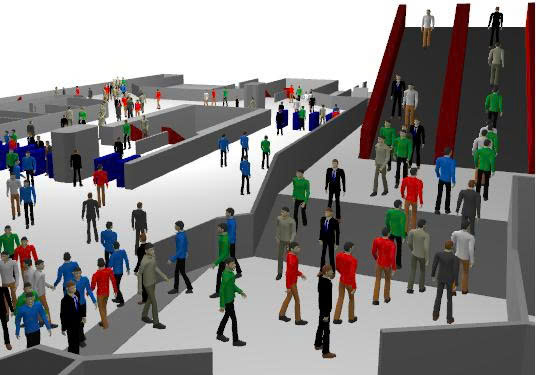
\includegraphics[
            width=\linewidth,
            height=0.67\textheight,
            keepaspectratio
        ]{pedestrian.jpg}
    \end{column}

    \hspace{0.015\textwidth}


    % Right: key ideas only
    \begin{column}{0.40\textwidth}
        \small
        \raggedright

        \vspace{0.08cm}

        \textbf{Two model families}

        \begin{itemize}
            \item \emph{Cellular automata}
            \item \emph{Continuous-space models}\\
            \vspace{0.1cm}
            $\Rightarrow$ Focus of this paper.
        \end{itemize}
    \end{column}

\end{columns}

\end{frame}


\begin{frame}{Introduction}

\vspace{-0.35cm}
\noindent{\large\bfseries Speed--Density Relation\par}

\vspace{0.08cm}

\begin{center}
    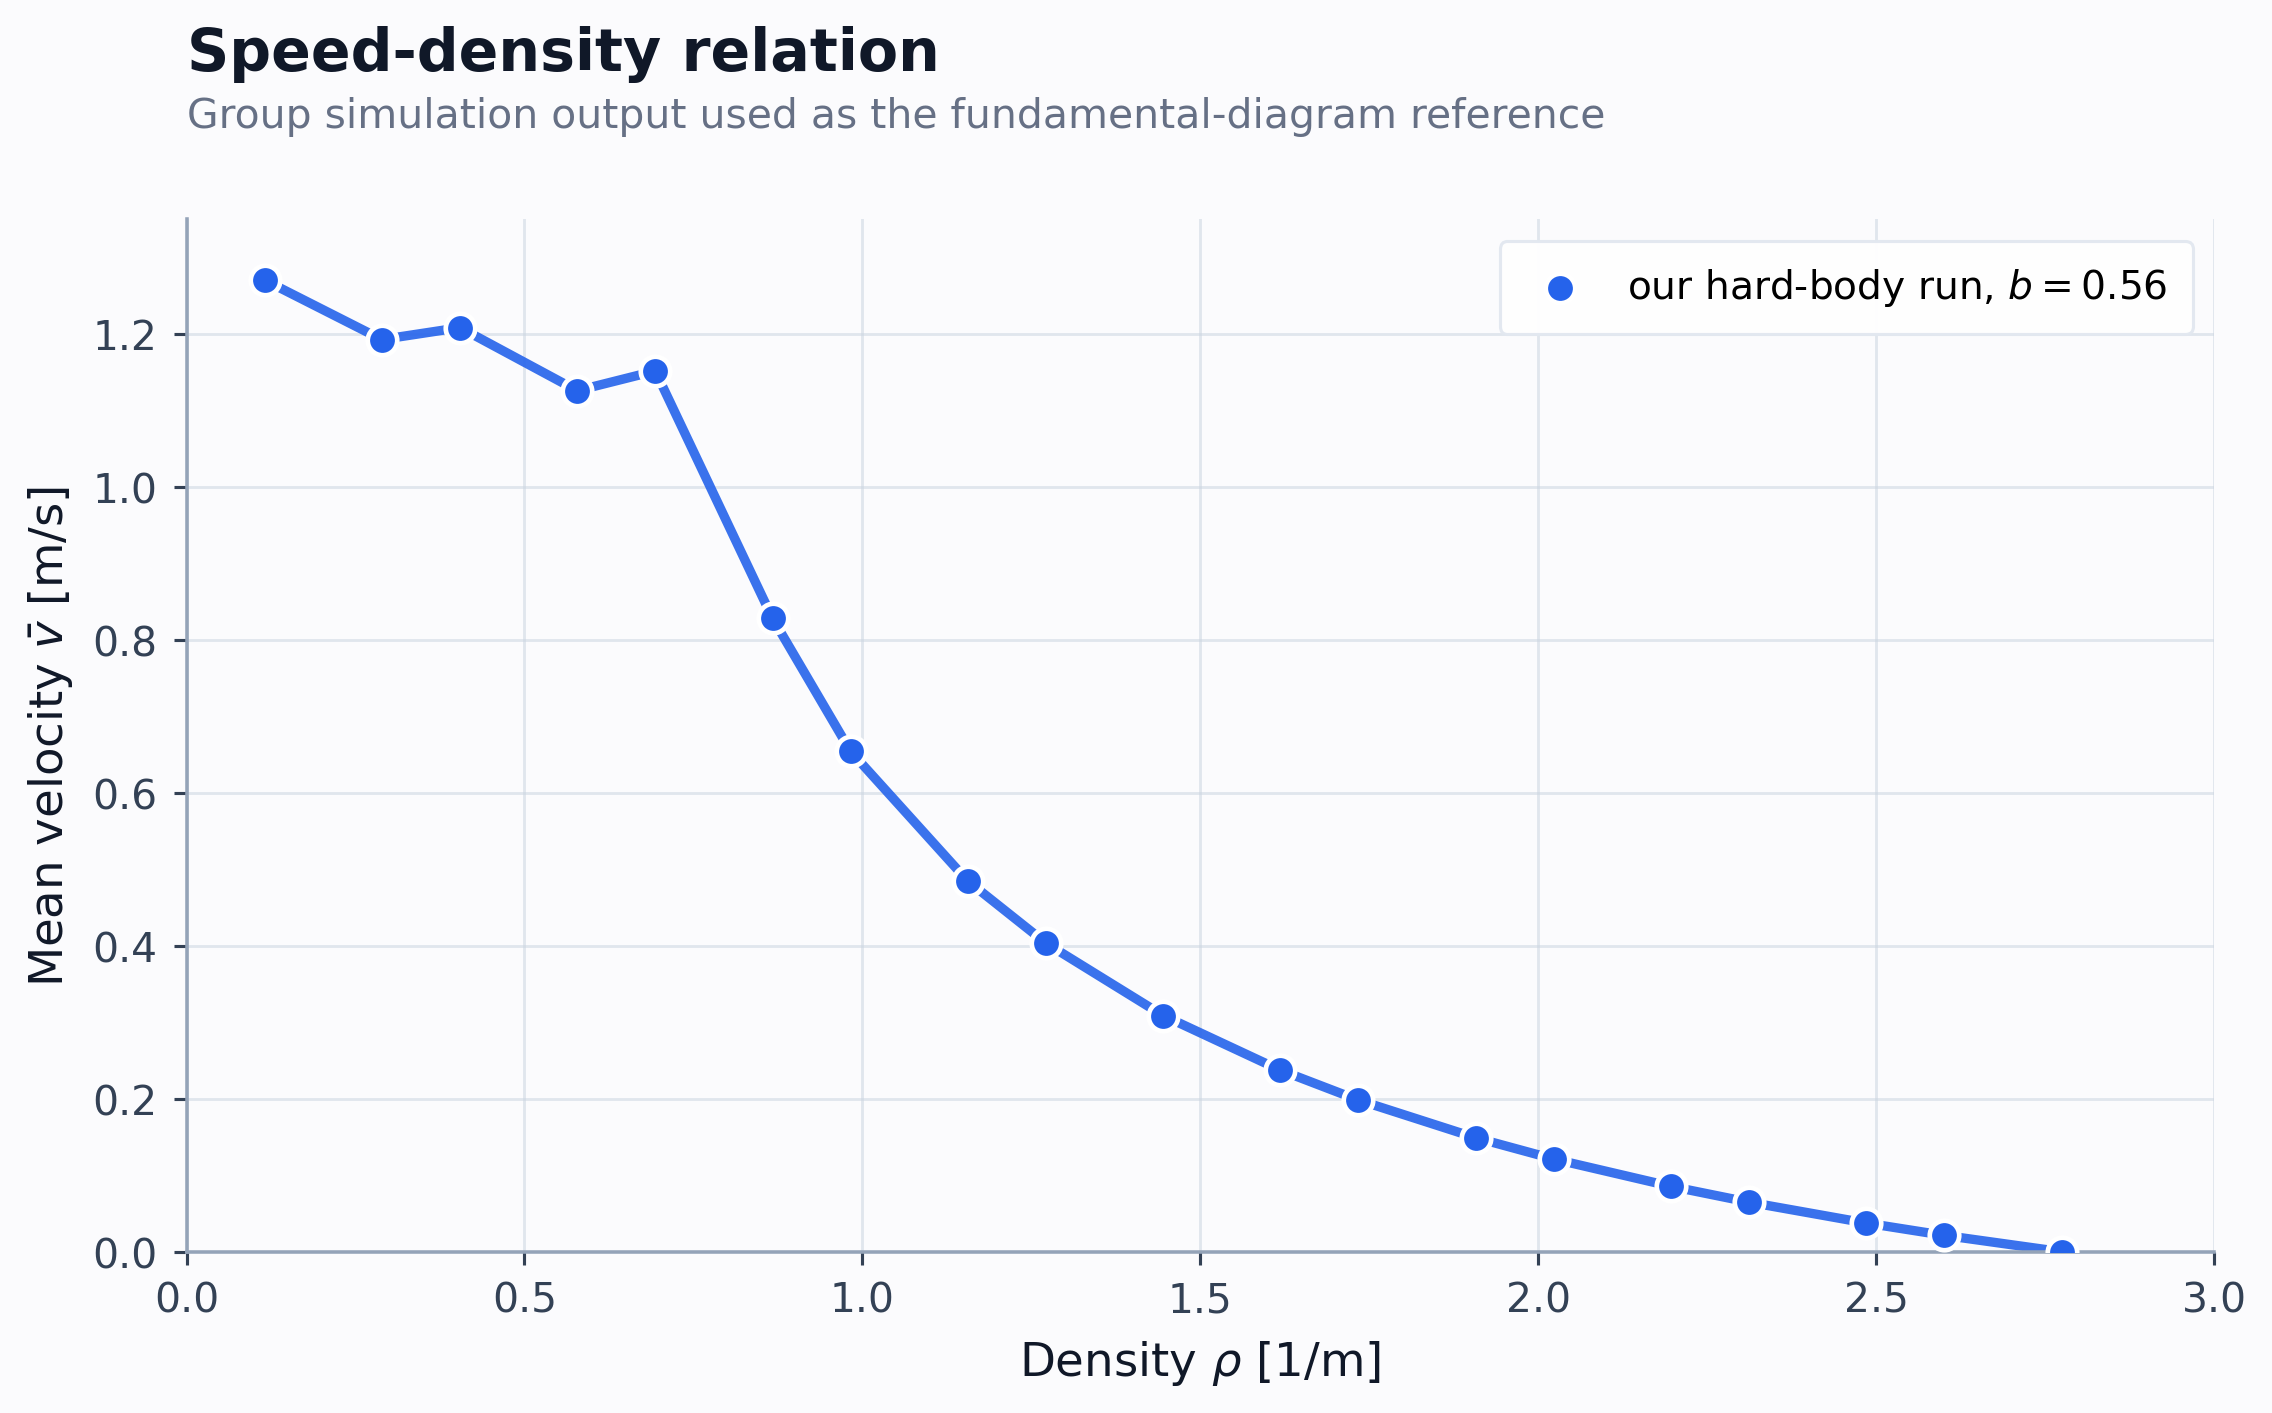
\includegraphics[
        width=0.48\textwidth,
        height=0.48\textheight,
        keepaspectratio
    ]{fundamental_diagram.png}

    \vspace{0.02cm}

    {\scriptsize
    \emph{Group simulation output: higher density $\Rightarrow$ lower mean walking speed.}
    }
\end{center}

\vspace{-0.05cm}

{\scriptsize
\raggedright

\begin{itemize}
    \setlength{\itemsep}{4pt}
    \setlength{\topsep}{2pt}

    \item \textbf{Fundamental diagram:} relationship between mean velocity
    $v$ and density $\rho$ reproduced by our 1D simulation.

    \item \textbf{Validation target:} a valid pedestrian model should
    reproduce the observed $v$--$\rho$ curve.
\end{itemize}
}

\end{frame}

\begin{frame}{Introduction}

\vspace{-0.55cm}
\noindent{\large\bfseries Why Use a 1D Model?\par}

\vspace{0.20cm}

\begin{center}
    {\Large
    \textbf{Single-file flow (1D)}
    \(\approx\)
    \textbf{Planar flow (2D)}
    }

    \vspace{0.06cm}

    {\scriptsize
    Similar speed--density behaviour: $v(\rho)$
    }
\end{center}

\vspace{0.12cm}

{\footnotesize
\raggedright

\begin{itemize}
    \setlength{\itemsep}{4pt}
    \setlength{\topsep}{2pt}

    \item \textbf{Empirical observation:} 1D and 2D pedestrian flows show
    similar velocity--density curves in both shape and magnitude.

    \item \textbf{Limited lateral effect:} lateral interactions do not
    noticeably change the fundamental diagram up to
    $\rho \approx 4.5\,\mathrm{m}^{-2}$.

    \item \textbf{Therefore:} a 1D model retains the essential macroscopic
    behaviour while isolating the effects of required space and interaction.
\end{itemize}
}

\end{frame}


\begin{frame}{Introduction: Research Objectives}
    \begin{itemize}
        \item \textbf{Paper:} Seyfried, Steffen \& Lippert, \emph{Basics of Modelling the Pedestrian Flow}, Physica A 368 (2006)
        \item \textbf{Main goal:} modify the 1D social force model so that it reproduces the empirical fundamental diagram
        \item \textbf{Two specific questions driving the modification:}
        \begin{enumerate}
            \item Does making the required space depend on velocity improve the fit to empirical data?
            \item How much does \emph{remote action} (a smooth repulsive force acting before contact) actually matter for the resulting $v$--$\rho$ curve?
        \end{enumerate}
    \end{itemize}
\end{frame}


% : Section 2: Motivation :
\section{Motivation}

\begin{frame}{Motivation: The Original Social Force Model}

\small
\raggedright

\setlength{\abovedisplayskip}{4pt}
\setlength{\belowdisplayskip}{4pt}
\setlength{\abovedisplayshortskip}{2pt}
\setlength{\belowdisplayshortskip}{2pt}

\vspace{0.10cm}

\textbf{Social Force Model:} Each pedestrian is modelled as a self-driven object in
continuous space, characterised by position $x_i(t)$, velocity $v_i(t)$,
and mass $m_i$.\\
For pedestrian $i$, its dynamics are described by:

\[
    \frac{dx_i}{dt}=v_i,
    \qquad
    m_i\frac{dv_i}{dt}=F_i
    =
    F_i^{drv}+F_i^{rep}
\]

\begin{itemize}
    \setlength{\itemsep}{4pt}
    \setlength{\topsep}{2pt}

    \item \textbf{Driving force} $F_i^{drv}$:
    drives pedestrian $i$ toward the intended velocity $v_i^0$.
    \[
        F_i^{drv}
        =
        m_i\frac{v_i^0-v_i}{\tau_i}
    \]

    \item \textbf{Repulsive force} $F_i^{rep}$:
    models the tendency to maintain personal space and prevent collisions
    through interactions with other pedestrians $j\neq i$.
    \[
        F_i^{rep}
        =
        \sum_{j\neq i}
        -\nabla
        A_i
            (\lVert x_j-x_i\rVert - d_i)^{-B_i}
    \]
\end{itemize}

\vspace{-0.05cm}

$\Rightarrow$ Even in this simple form, the model can reproduce collective
effects such as lane formation and oscillations at bottlenecks.

\end{frame}

\begin{frame}{Motivation: Why Modify the Model for 1D?}

{\footnotesize
\raggedright
\setlength{\baselineskip}{0.90\baselineskip}

In a single-file setting, the original interaction needs to be adapted:

\vspace{0.12cm}

\begin{columns}[T,onlytextwidth]

    % Left: motion direction and interaction scope
    \begin{column}{0.47\textwidth}

        \textbf{1. Physically valid motion}

        A symmetric repulsion may cause backward motion
        $(v_i < 0)$ or accelerate a pedestrian beyond their intended
        speed $(v_i > v_i^0)$.

        \vspace{0.25cm}

        \textbf{2. Front-only influence}

        In single-file walking, motion should be governed by the
        pedestrian directly ahead, not by pedestrians behind.

    \end{column}

    \hfill

    % Right: required space
    \begin{column}{0.48\textwidth}

        \textbf{3. Speed-dependent required space}

        A fixed required length does not reproduce the empirical
        velocity--density relation correctly.

        \vspace{0.12cm}

        The required length should increase with walking speed:

        \[
            d_i(t)=a_i+b_i v_i(t)
        \]

        \vspace{0.05cm}

        This captures the fact that faster pedestrians require more
        space in front of them.

    \end{column}

\end{columns}

\vspace{0.18cm}

\[
\boxed{
\text{Forward-only interaction}
\quad + \quad
\text{speed-dependent required space}
}
\]

\vspace{0.05cm}

$\Rightarrow$ The reduced 1D model isolates how required space and
remote interaction shape the fundamental diagram.

}

\end{frame}

% : Section 3: Methodology :
\section{Methodology}

\begin{frame}{Methodology: Problem Setting and Mathematical Model}
    \begin{itemize}
        \item \textbf{Setup:} $N$ pedestrians confined to a 1D corridor of length $L$, with periodic boundary conditions
        \item \textbf{Ordering convention:} pedestrians are indexed so that $i{+}1$ is always the one immediately ahead, i.e. $x_{i+1}(t) > x_i(t)$; all masses normalized to $m_i = 1$
        \item \textbf{Density:} $\rho = N/L$
        \item \textbf{Equation of motion for each pedestrian:}
        \[
            \frac{dx_i}{dt} = v_i(t), \qquad \frac{dv_i}{dt} = F_i(t)
        \]
        \item \textbf{Key departure from the original model:} $F_i(t)$ is no longer a superposition $\sum_{j\neq i} F_{ij}$ over every other pedestrian
        \begin{itemize}
            \item Instead, $F_i(t)$ is determined \textbf{exclusively} by the state of pedestrian $i+1$ in front
        \end{itemize}
        \item This single change in scope is what allows the system to be analyzed and simulated as a chain of one-sided, local interactions rather than a fully coupled many-body force field
    \end{itemize}
\end{frame}


\begin{frame}{Methodology: Modifications to the Social Force Model}
    \begin{itemize}
        \item \textbf{Modification 1 : One-sided (forward-only) interaction}
        \begin{itemize}
            \item The sum $\sum_{j\neq i}$ is collapsed into a single term involving only pedestrian $i+1$
            \item In single-file motion, a person's pace is dictated by the gap ahead, not by anyone behind
        \end{itemize}
        \item \textbf{Modification 2 : Hard velocity bound}
        \begin{itemize}
            \item Resulting velocity is restricted to the physically sensible range $v_i \in [0,\, v_i^0]$
            \item Lower bound at $0$: rules out backward motion induced by repulsion
            \item Upper bound at $v_i^0$: rules out being "pushed" faster than one's own intended speed
        \end{itemize}
        \item \textbf{Modification 3 : Required length as a function of velocity}
        \begin{itemize}
            \item The fixed hard-core size $d_i$ is replaced by a quantity that grows with current speed:
            \[
                d_i(t) = a_i + b_i\, v_i(t)
            \]
            \item Captures the empirical fact that a faster-moving pedestrian occupies more space along the direction of travel
        \end{itemize}
    \end{itemize}
\end{frame}


\begin{frame}{Interaction Force Models: Hard body (no remote action)}
    \begin{itemize}
        \item \textbf{Force law:}
        \[
            F_i(t) =
            \begin{cases}
                \dfrac{v_i^0 - v_i(t)}{\tau_i}, & x_{i+1}(t) - x_i(t) > d_i(t) \\[10pt]
                -\,\delta(t)\,v_i(t), & x_{i+1}(t) - x_i(t) \le d_i(t)
            \end{cases}
        \]
        with $d_i(t) = a_i + b_i\,v_i(t)$
        \item Depends on exactly three quantities: pedestrian $i$'s own position and velocity, and the position $x_{i+1}$ of the one ahead
        \item \textbf{Free regime} (gap $> d_i$): only the driving term acts, pedestrian accelerates toward $v_i^0$
        \item \textbf{Contact regime} (gap $\le d_i$): velocity is forced to zero --- an instantaneous switch, not a smooth decay
        \item Since $d_i$ scales with $v_i$, a faster pedestrian needs more space
        \item There is no anticipation built in: the model reacts only once the threshold is actually crossed, never before
    \end{itemize}
\end{frame}


\begin{frame}{Interaction Force Models: Hard body (with remote action)}
    \begin{itemize}
        \item \textbf{Force law:}
        \[
            F_i(t) =
            \begin{cases}
                G_i(t), & v_i(t) > 0 \\[4pt]
                \max\big(0,\, G_i(t)\big), & v_i(t) \le 0
            \end{cases}
        \]
        \[
            G_i(t) = \underbrace{\frac{v_i^0 - v_i(t)}{\tau_i}}_{\text{driving}} \;-\; \underbrace{e_i\left(\frac{1}{x_{i+1}(t)-x_i(t)-d_i(t)}\right)^{f_i}}_{\text{remote repulsion}}
        \]
        \item Still strictly one-sided: only the pedestrian ahead contributes to $G_i$
        \item The repulsive term grows without bound as the gap approaches $d_i(t)$, so deceleration begins \textbf{before} contact is actually made
        \item $e_i$ sets the strength of the repulsion; $f_i$ sharpness as gap narrows
        \item  Stopped pedestrian cannot be pushed backward.
        \item Consequence: with $e_i, f_i$ properly tuned, full stops happen mainly during the early relaxation phase, far less often.
    \end{itemize}
\end{frame}


\begin{frame}{Time Stepping: Hard body with Remote Action}
    \begin{columns}[T] % [T] giúp căn lề trên cùng cho cả 2 cột

        % Cột bên trái: Chữ và công thức
        \begin{column}{0.55\textwidth}
            \begin{itemize}
                \item \textbf{Why it is simple here:} $G_i(t)$ is continuous along the trajectory
                \item \textbf{Scheme used: explicit Euler}, with $\Delta t = 0.001\ \mathrm{s}$:
                \[
                    v_i(t+\Delta t) = v_i(t) + \Delta t \cdot F_i(t)
                \]
                \[
                    x_i(t+\Delta t) = x_i(t) + \Delta t \cdot v_i(t+\Delta t)
                \]
                \item Since $\Delta t$ is small relative to how fast inter-pedestrian gaps actually change, the standard Euler discretization error stays negligible

            \end{itemize}
        \end{column}

        % Cột bên phải: Ảnh
        \begin{column}{0.45\textwidth}
            \begin{figure}
                \centering
                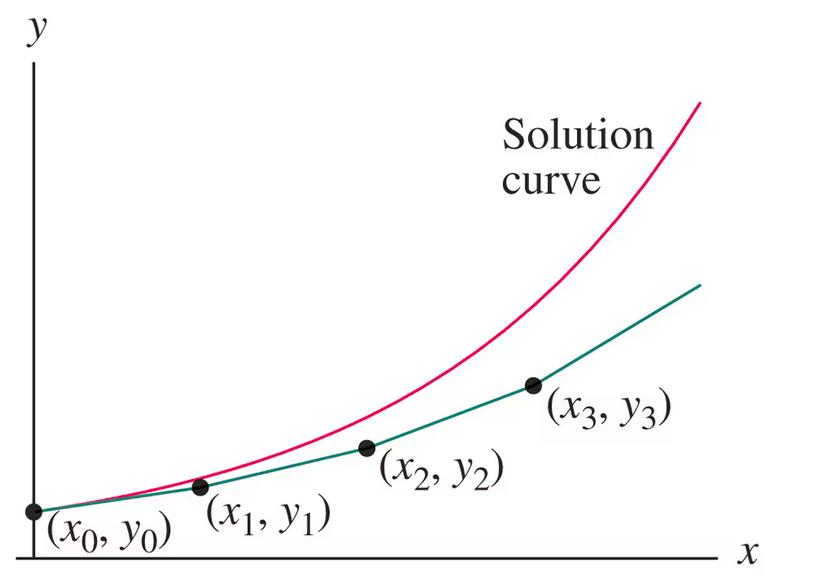
\includegraphics[width=\textwidth]{eulermethod1.jpg}
                \caption{Example of Euler's method}
            \end{figure}
        \end{column}

    \end{columns}
\end{frame}


\begin{frame}{Time Stepping: Hard body without Remote Action --- The Problem}
    \begin{columns} % Thêm tuỳ chọn [T] sau \begin{columns} nếu bạn muốn căn lề trên cùng cho cả 2 bên

        % Cột bên trái: Ảnh
        \begin{column}{0.45\textwidth}
            \begin{figure}
            \centering
            % Lưu ý: để width=\textwidth ở đây nghĩa là bằng 100% chiều rộng của cột chứa nó
            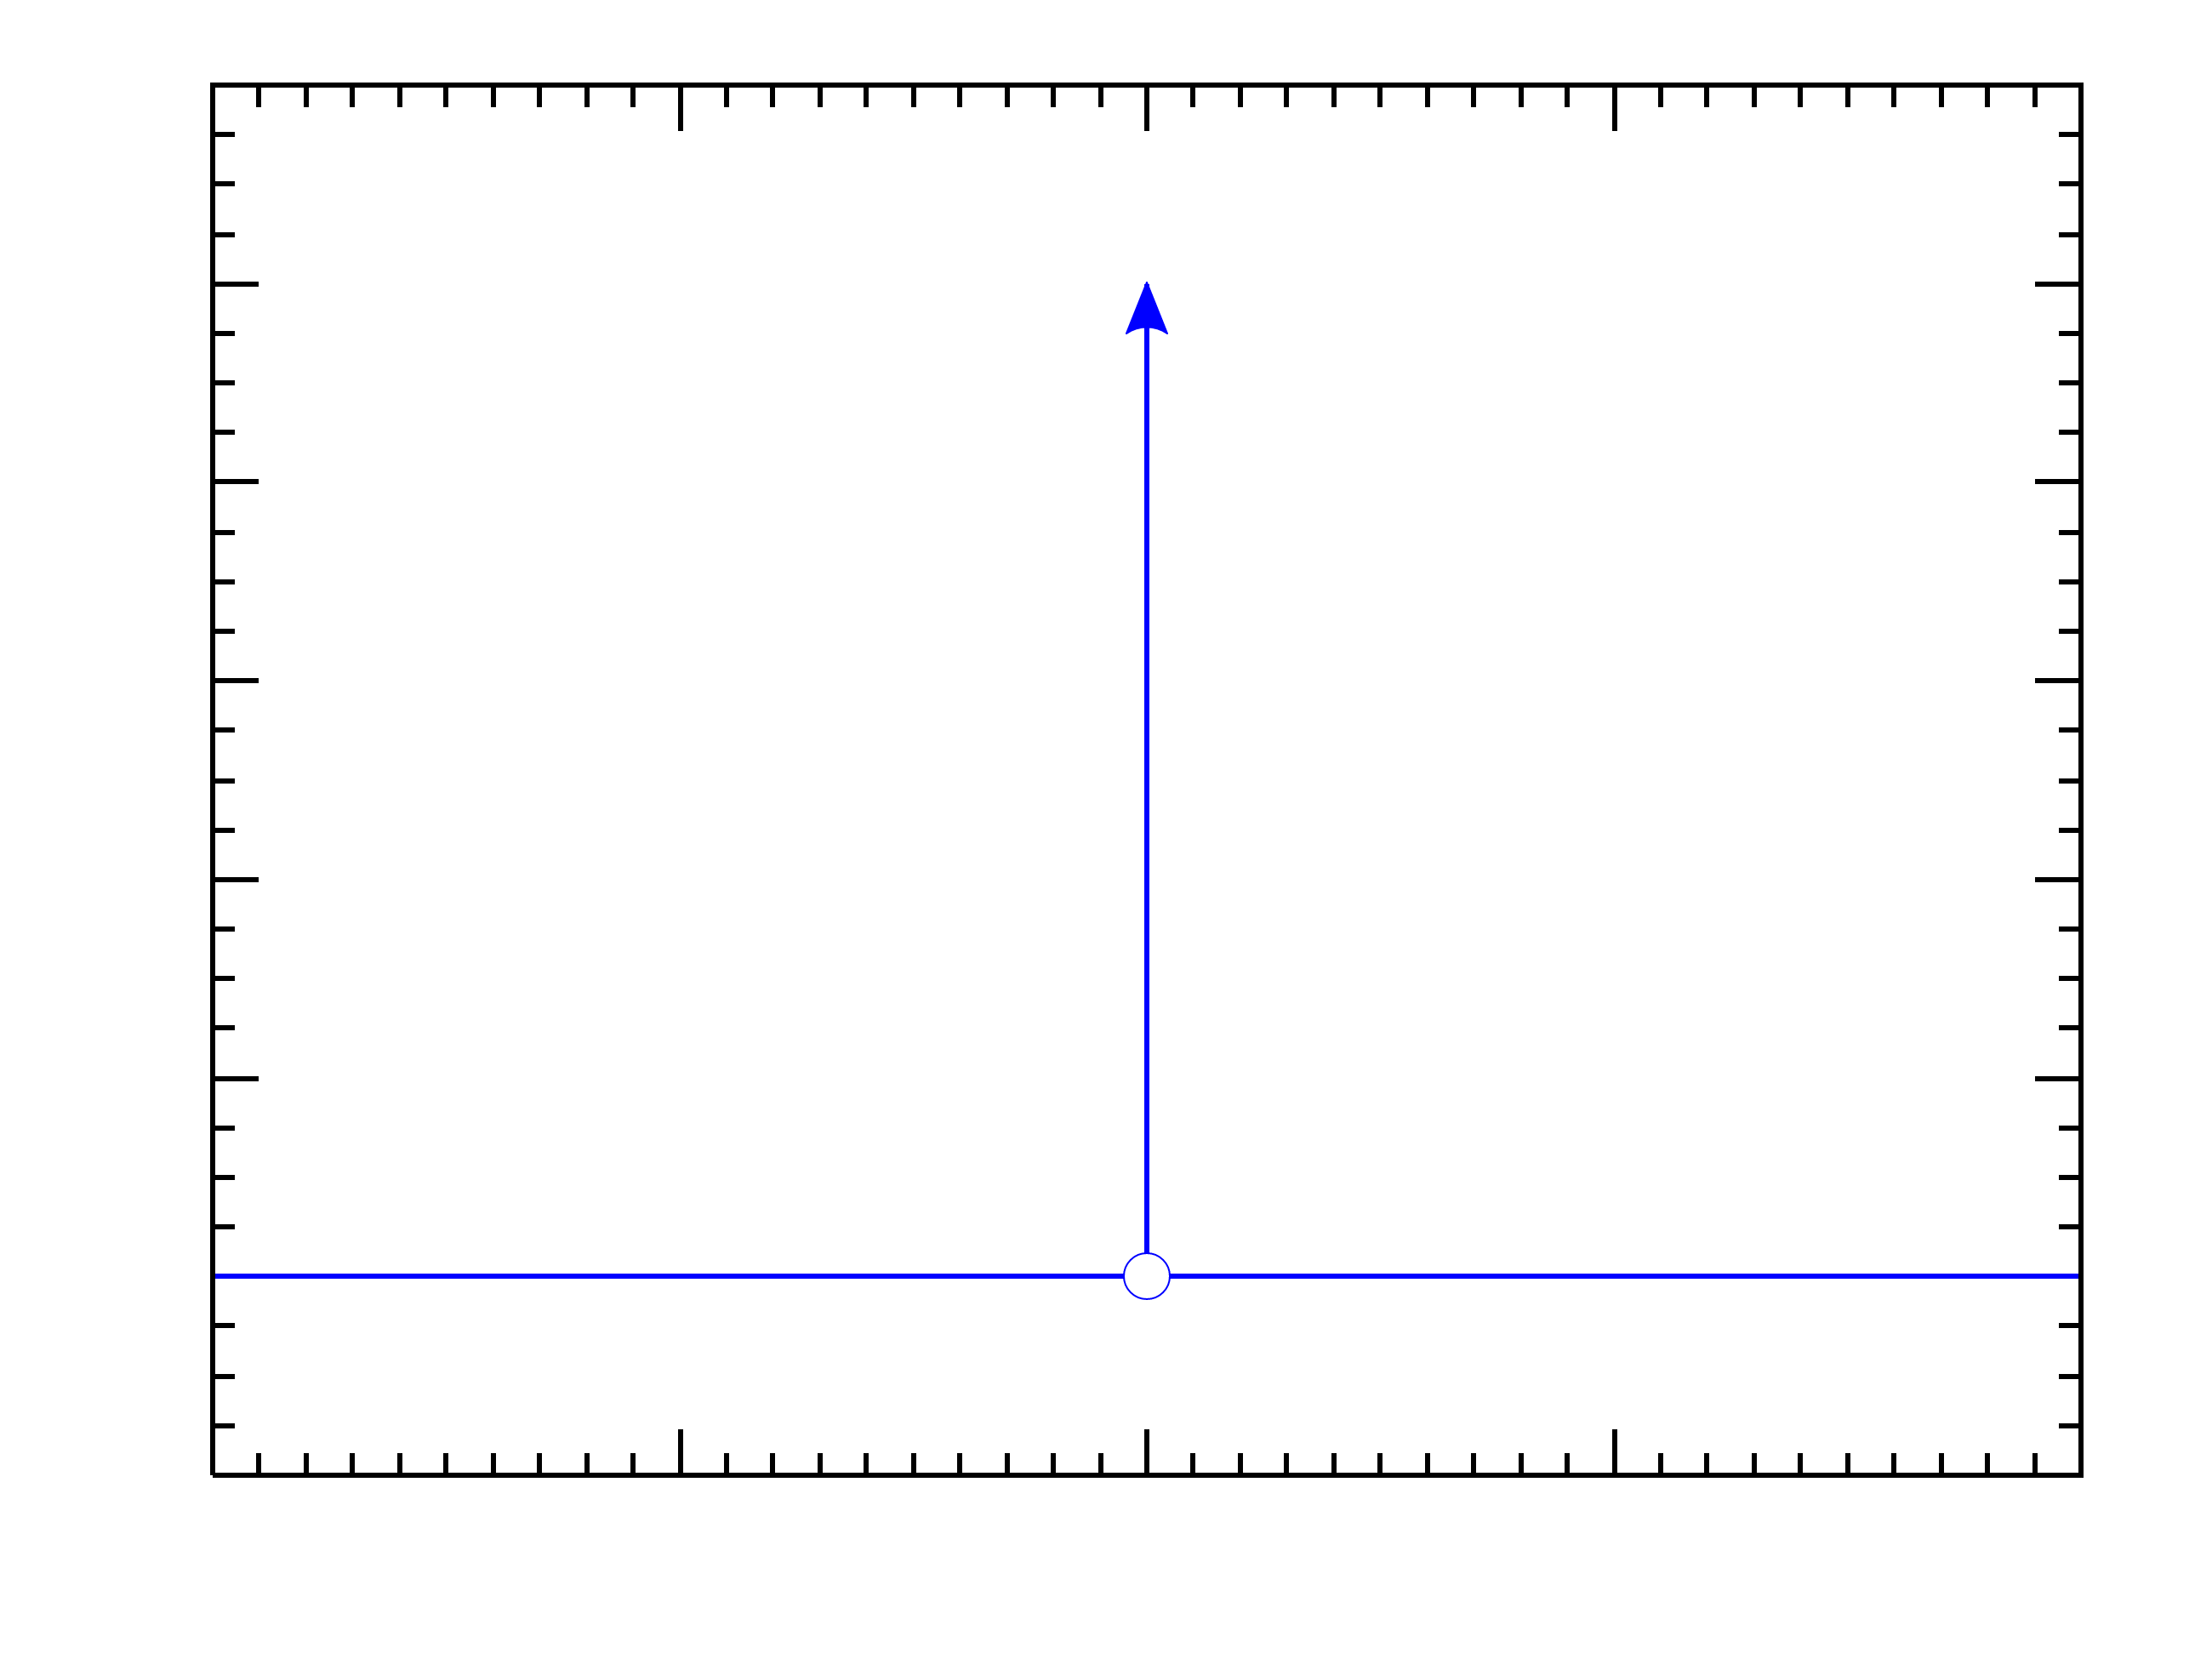
\includegraphics[width=\textwidth]{Dirac_distribution_PDF.png}
            \caption{Dirac spikes at collision times $t^*$ are unknown until the trajectory is solved}
            \end{figure}
        \end{column}

        % Cột bên phải: Chữ
        \begin{column}{0.55\textwidth}
            \begin{itemize}
                \item $F_i$ is \textbf{discontinuous}: switches abruptly between driving term and stop

                \item A jump in $v_i$ at collision time $t^*$ means $\dfrac{dv_i}{dt}$ contains a \textbf{Dirac spike}.
                \begin{itemize}
                    \item The RHS is a \emph{distribution}, not a regular function - standard ODE solvers cannot handle it directly
                \end{itemize}
                \item The exact collision time $t^*$ is \textbf{not known in advance}.
            \end{itemize}
        \end{column}

    \end{columns}
\end{frame}

\begin{frame}{Time Stepping: Corrective Algorithm (Steps 1--3)}
    \textbf{Key idea:} predict first with plain Euler, then fix any violations afterward
    \vspace{0.4em}
    \begin{enumerate}
        \item \textbf{Predict} : update every pedestrian as if unconstrained:
        \[
            v_i^{new} = v_i + \Delta t \cdot \frac{v_i^0 - v_i}{\tau_i}, \qquad
            x_i^{new} = x_i + \Delta t \cdot v_i^{new}
        \]

        \item \textbf{Check} : compute spacing for every pair $(i,\, i{+}1)$:
        \[
            s_i = x_{i+1}^{new} - x_i^{new}
        \]

        \item \textbf{Correct} : if $s_i \le d_i$, undo pedestrian $i$'s move and stop them:
        \[
            x_i^{new} \leftarrow x_i^{old}, \qquad v_i^{new} \leftarrow 0
        \]
        \begin{itemize}
            \item Pedestrian $i$ is projected back to its last valid position
        \end{itemize}
    \end{enumerate}
\end{frame}


\begin{frame}{Time Stepping: Corrective Algorithm (Steps 4--5)}
    \begin{enumerate}
        \setcounter{enumi}{3}
        \item \textbf{Propagate}: re-examine the pedestrian directly behind $i$
        \begin{itemize}
            \item Rolling $i$ back to $x_i^{old}$ shrinks the gap for pedestrian $i{-}1$:
            \[
                s_{i-1} = x_i^{old} - x_{i-1}^{new} \quad \longrightarrow \quad \text{may now violate } s_{i-1} \le d_{i-1}
            \]
            \item If so, apply Step 3 to $i{-}1$ as well, then check $i{-}2$, and so on
        \end{itemize}

        \item \textbf{Iterate} : repeat Steps 3--4 until no overlap remains:
        \[
            s_i > d_i \quad \forall\, i
        \]
    \end{enumerate}
    \vspace{0.5em}
    \begin{block}{Why propagation matters}
        Freezing one pedestrian can trigger a \emph{cascade} of corrections down the queue - especially under periodic boundary conditions, where the chain wraps around the entire system.
    \end{block}
\end{frame}

\begin{frame}{Time Stepping: Corrective Algorithm --- Visual Summary}
    \begin{figure}
        \centering
        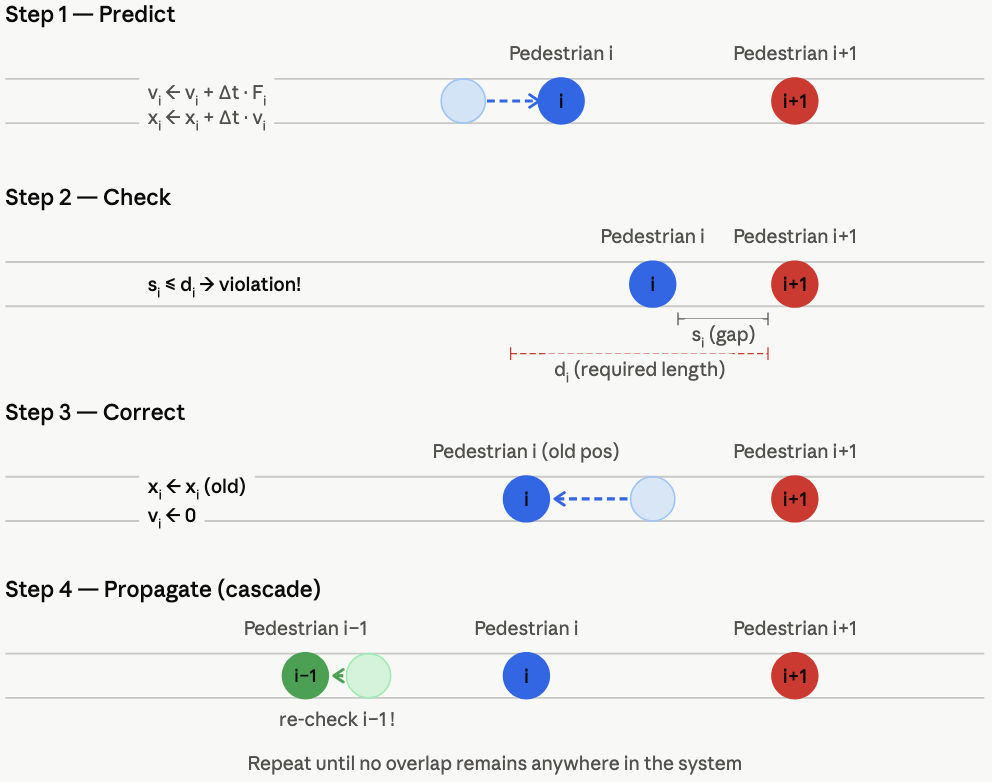
\includegraphics[width=0.85\textwidth, height=0.82\textheight, keepaspectratio]{algo_with_out_remote.png}
    \end{figure}
\end{frame}


% \begin{frame}{Time Stepping: Why This Approximation is Acceptable}
%     \begin{itemize}
%         \item \textbf{What makes it an approximation:}
%         \begin{itemize}
%             \item The true collision time $t^*$ lies \emph{inside} the interval $(t_k,\, t_k {+} \Delta t)$, but the algorithm treats it as if it happened at the \emph{end} of the step
%             \item Corrections are applied sequentially (one pedestrian at a time), not simultaneously as physics would require
%         \end{itemize}

%         \item \textbf{Why the error is small:}
%         \begin{itemize}
%             \item Timing error is $O(\Delta t)$ per collision --- with $\Delta t = 0.001$ s, positions shift by at most $\sim 1$ mm per step
%             \item The sequential ordering introduces an artifact, but its effect on macroscopic statistics $\bar{v}(\rho)$ is negligible
%         \end{itemize}

%         % \item \textbf{Verified empirically:} simulations were re-run with different ordering of pedestrians
%         % \[
%         %     \text{differences} \approx O(\text{floating-point rounding}) \quad \checkmark
%         % \]

%         % \item \textbf{Bottom line:} the approximation is far cheaper than exact event detection, and accurate enough for the macroscopic quantity of interest --- the fundamental diagram
%     \end{itemize}
% \end{frame}

% : Section 5: Experiments and Results :
\section{Experiments and Results}
\begin{frame}{Simulation Setup}
\small
\begin{itemize}
    \item \textbf{Environment:} Periodic boundary conditions, length $L=17.3\,\mathrm{m}$.
    \item \textbf{Input Parameters:}
    \begin{itemize}
        \item \textbf{Intended velocity:} $v \approx$ normal distribution with $\mu=1.24$, $\sigma=0.05\,\mathrm{m/s}$.
        \item \textbf{Relaxation time:} $\tau=0.61\,\mathrm{s}$.
        \item \textbf{Minimum stationary space:} $a=0.36\,\mathrm{m}$.
    \end{itemize}
    \item \textbf{Simulation Protocol:}
    \begin{itemize}
        \item Beginning with $3\times10^5$ relaxation steps.
        \item Then $3\times10^5$ measurement steps.
    \end{itemize}
    \item \textbf{Empirical data:} Extracted via plot digitization from Seyfried et al. (2005) reference.
\end{itemize}
\end{frame}

\begin{frame}{Hard-body Model without Remote Action}
\small
\begin{columns}[T,onlytextwidth]
    % Left Column: Analysis
    \begin{column}{0.5\textwidth}
        \textbf{Space-Velocity Coupling ($b$):}
        \begin{itemize}
            \item \textbf{Constant Space ($b = 0$):}
            \begin{itemize}
                \item Fails to replicate empirical trends.
                \item \alert{Incorrect curvature}: sharp velocity drop at low densities.
            \end{itemize}

            \vspace{0.2cm}

            \item \textbf{Dynamic Space ($b > 0$):}
            \begin{itemize}
                \item Restores characteristic \textbf{convex shape}.
                \item \textbf{Optimal fit}: $b = 0.56\,\mathrm{s}$ (Seyfried data).
            \end{itemize}
        \end{itemize}
    \end{column}

    % Right Column: Diagram and finding
    \begin{column}{0.48\textwidth}
        \centering
        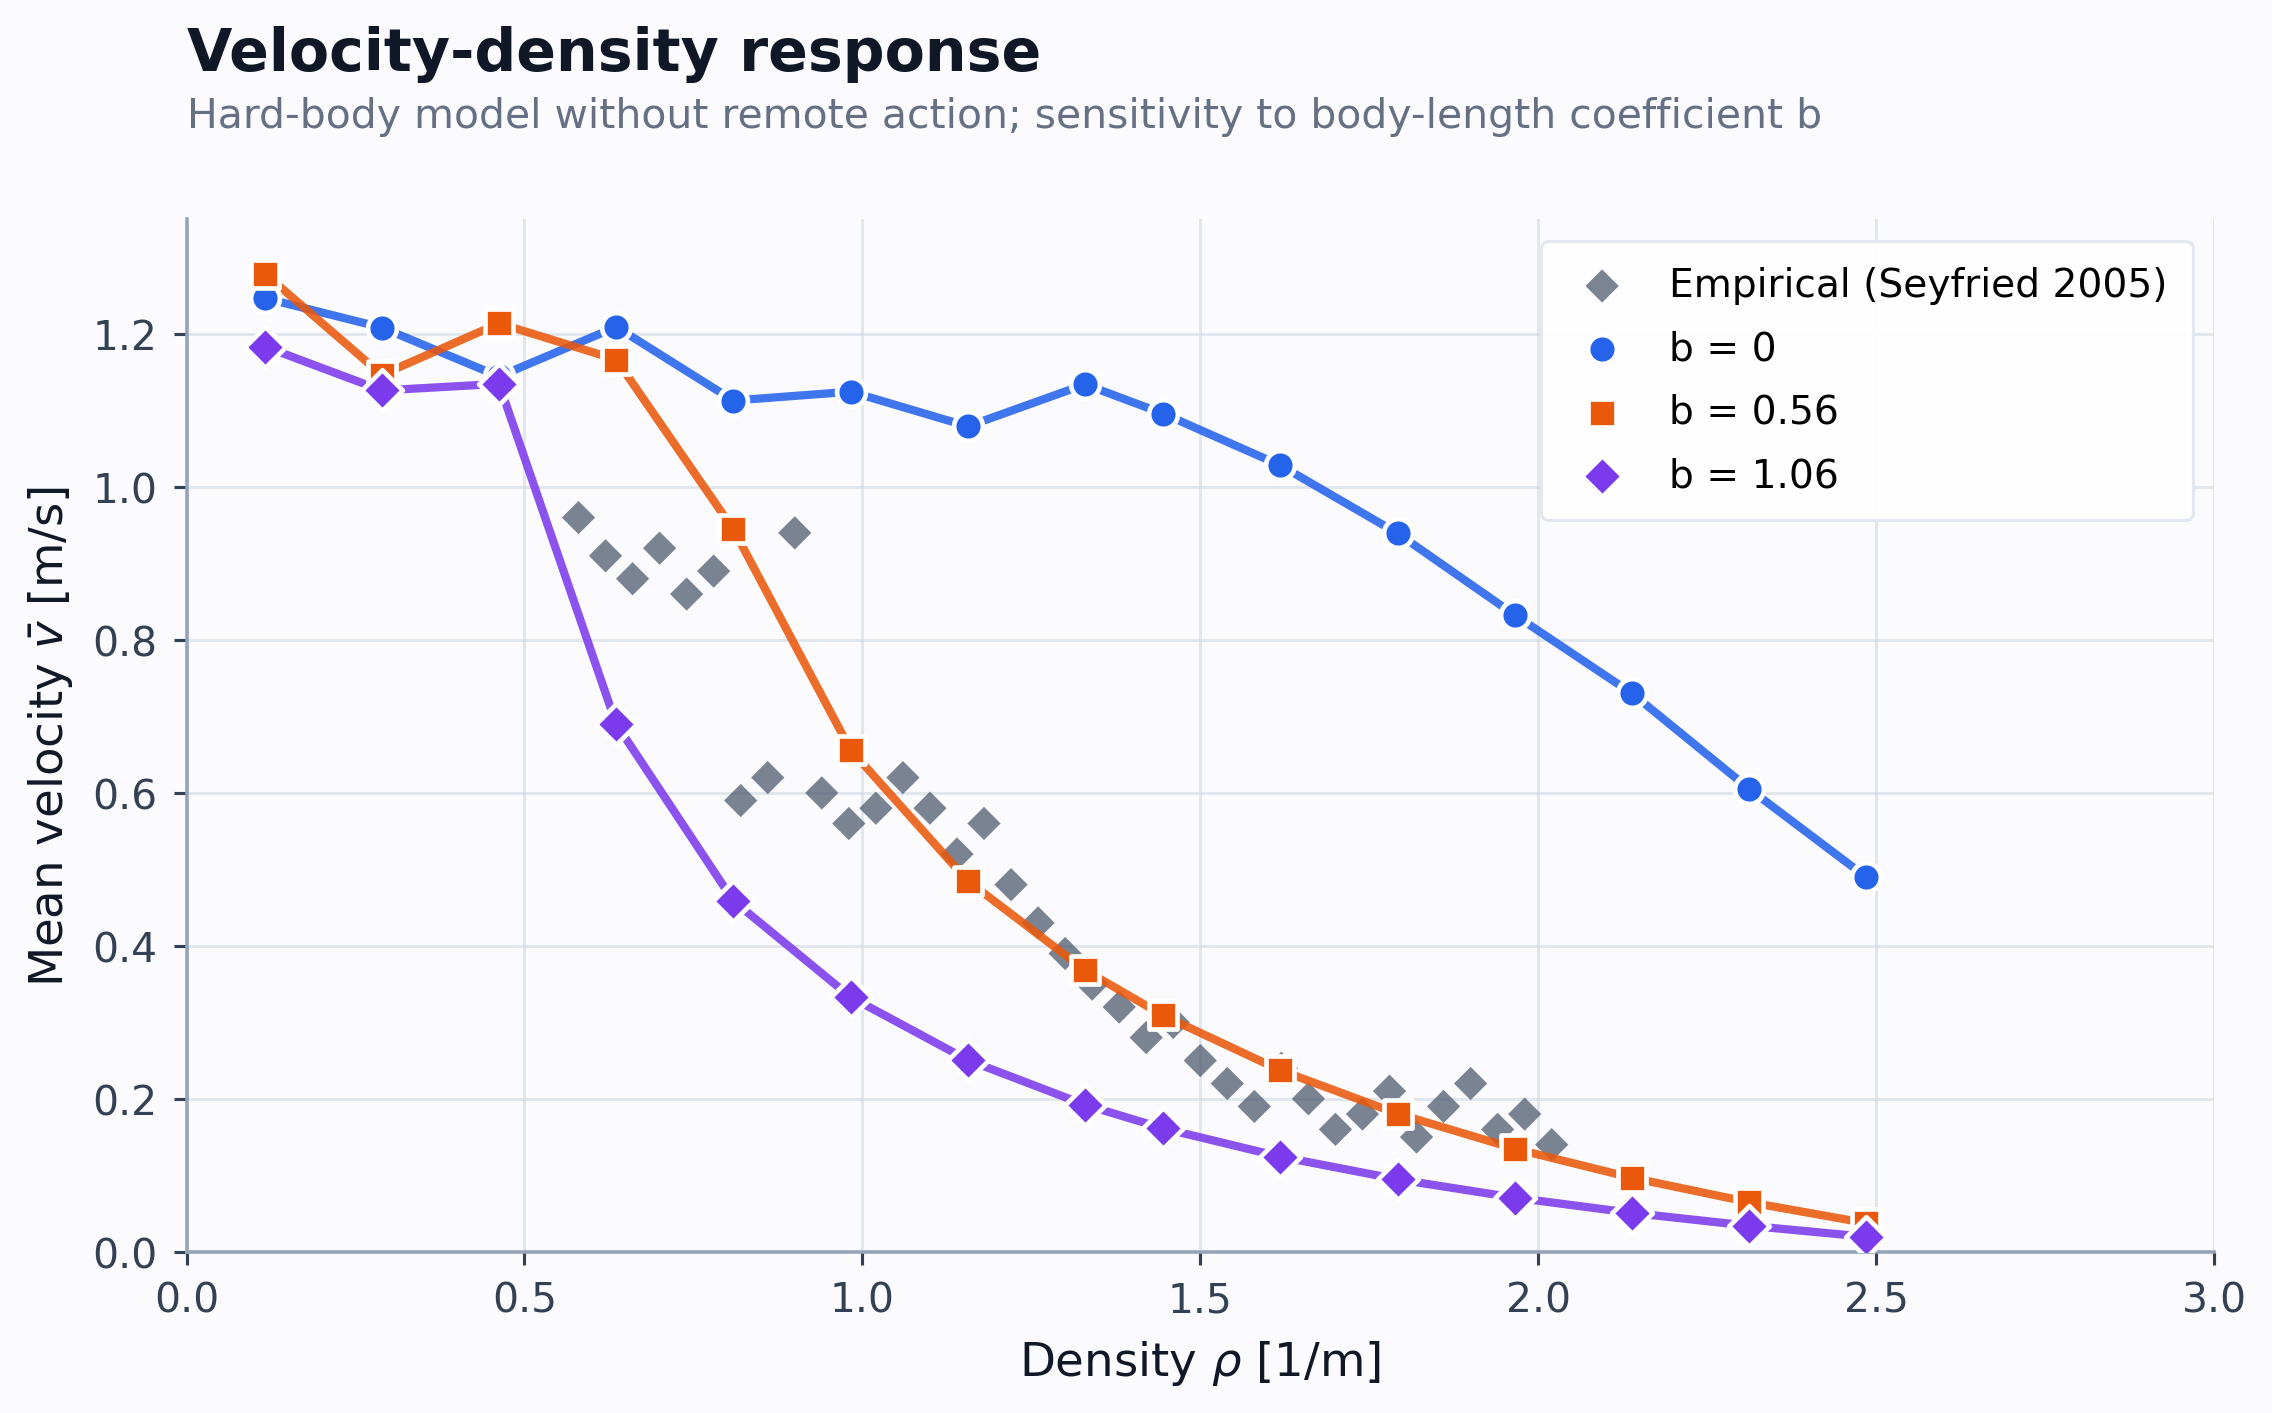
\includegraphics[width=\linewidth, height=0.48\textheight, keepaspectratio]{no_remote_action.png}
        \vspace{0.08cm}
        {\scriptsize \par \emph{Fig 1: Impact of parameter $b$ with Seyfried empirical points.}}
        \vspace{0.12cm}
        \begin{block}{Key Finding}
            Empirical data is \textbf{only reproducible} if required space ($d$) scales with velocity ($b > 0$).
        \end{block}
    \end{column}
\end{columns}
\end{frame}

\begin{frame}{Hard-body Model with Remote Action}
\small
\begin{columns}[T,onlytextwidth]
    % Left Column: Diagram
    \begin{column}{0.48\textwidth}
        \centering
        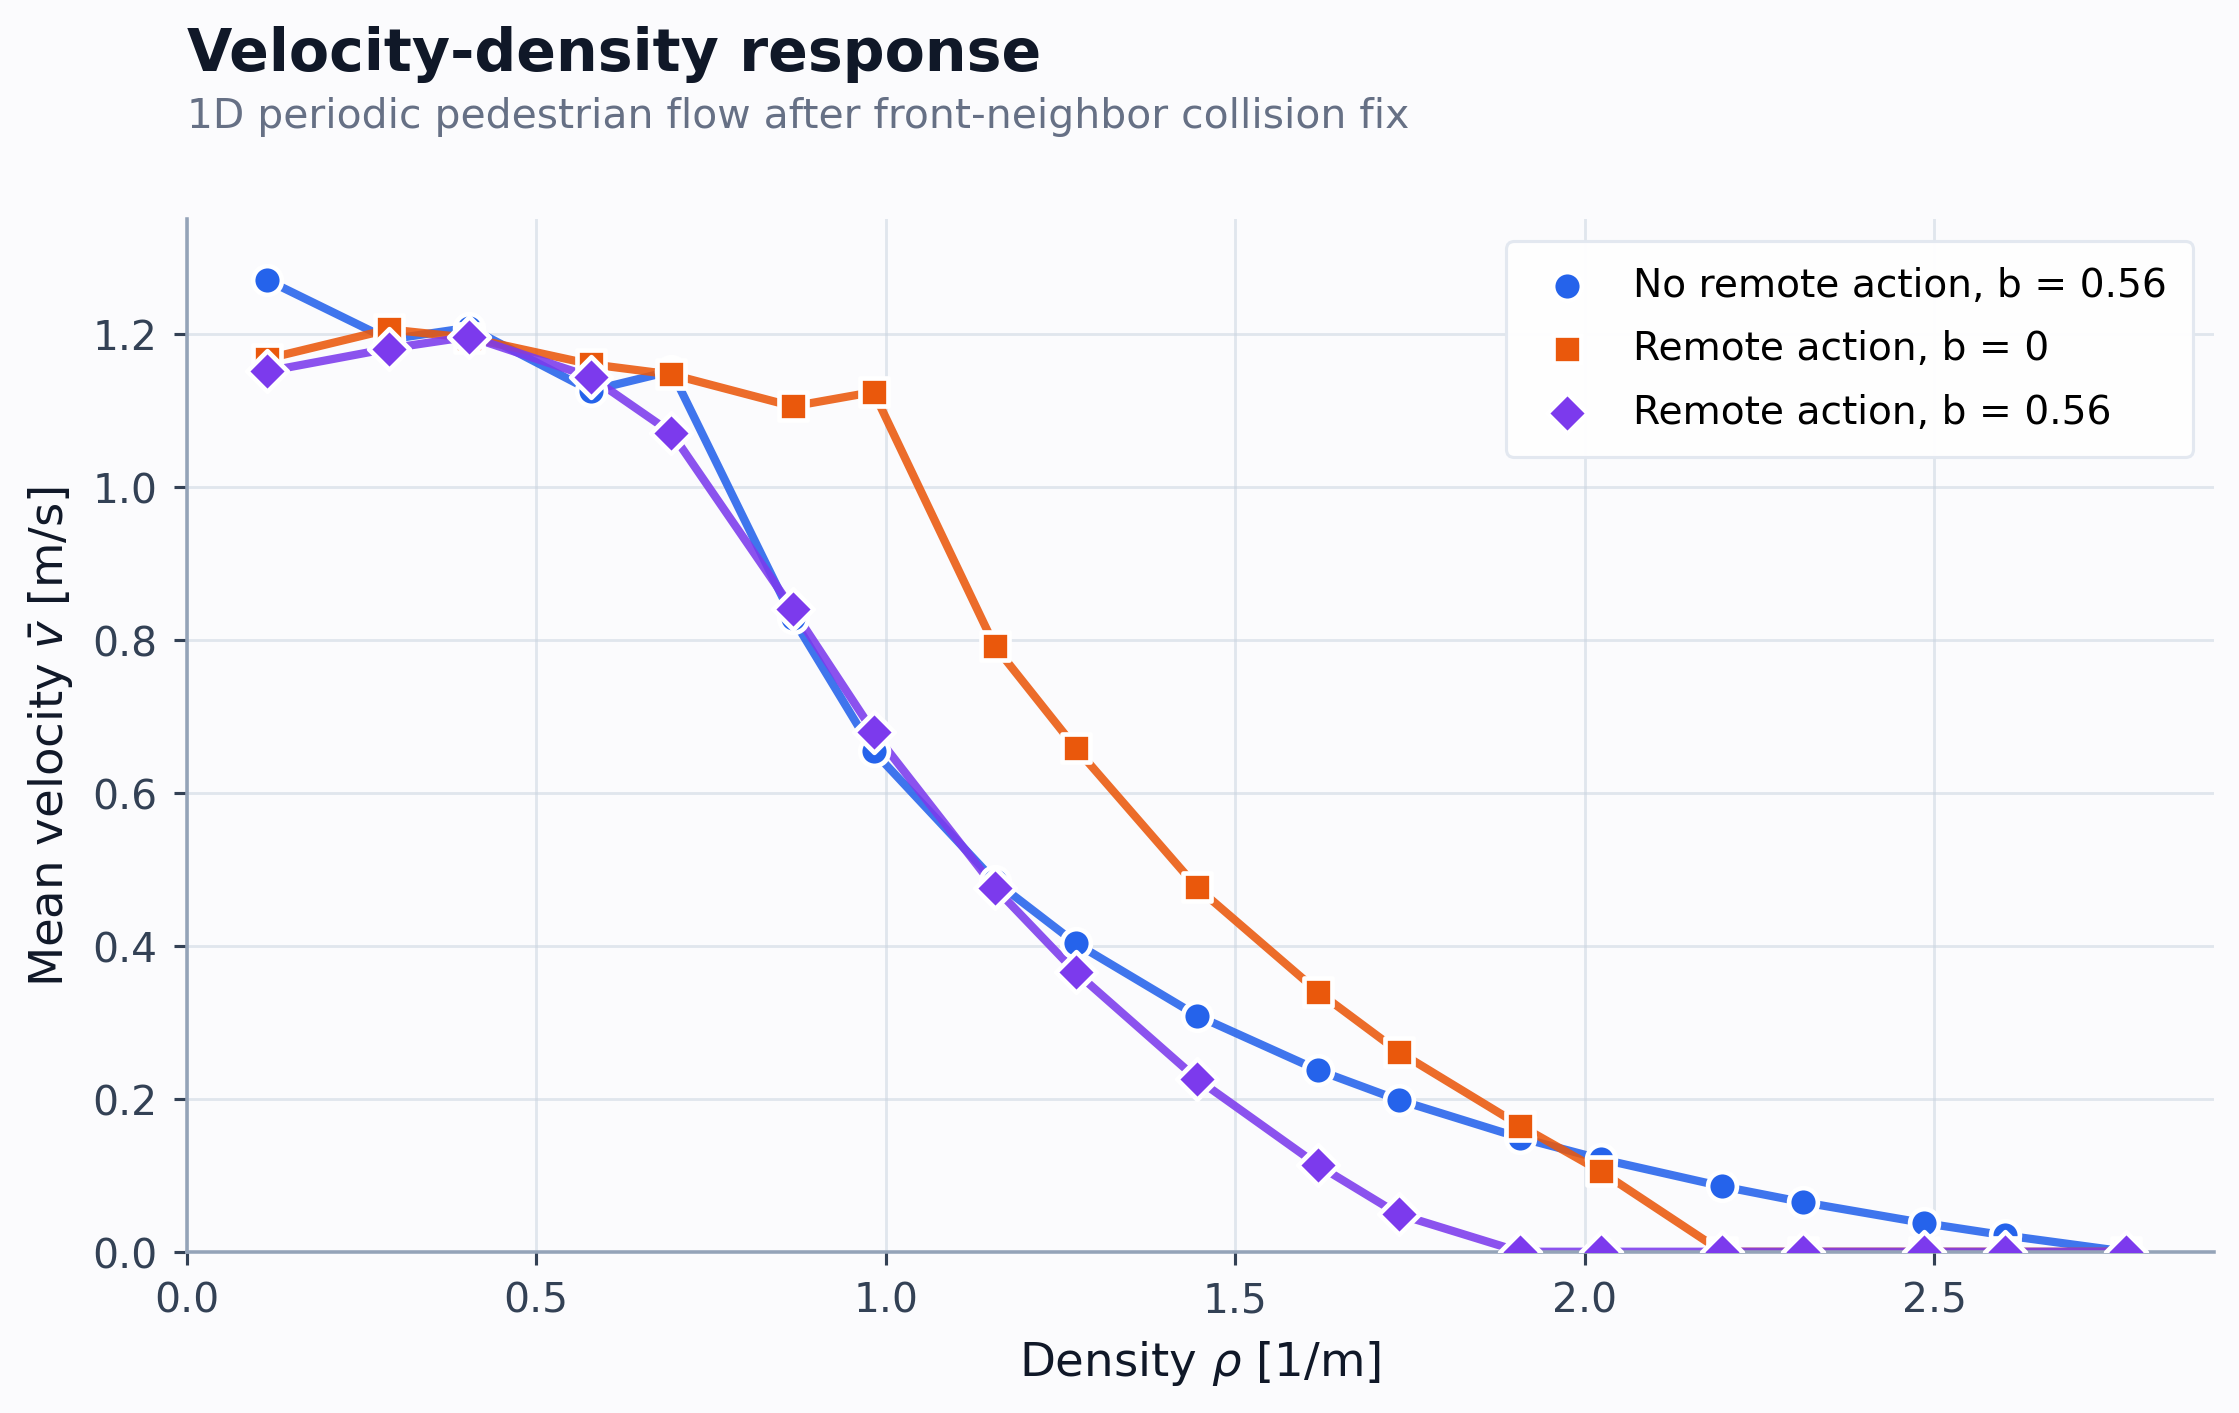
\includegraphics[width=\linewidth, height=0.65\textheight, keepaspectratio]{remote_action.png}
        \vspace{0.1cm}
        {\scriptsize \par \emph{Fig 2: $v$--$\rho$ curves with remote forces.}}
    \end{column}

    % Right Column: Analysis
    \begin{column}{0.5\textwidth}
        \textbf{Impact of Remote Forces:}
        \begin{itemize}
            \item \textbf{Dynamic Space ($b = 0.56\,\mathrm{s}$):}
            \begin{itemize}
                \item \textbf{Negligible effect} on macro diagram.
                \item Identical to model without remote action.
            \end{itemize}

            \vspace{0.2cm}

            \item \textbf{Constant Space ($b = 0$):}
            \begin{itemize}
                \item Unphysical \textbf{"velocity gap"} at $\rho \approx 1.2\,\mathrm{m}^{-1}$.
                \item Flow drops abruptly to near-zero.
            \end{itemize}
        \end{itemize}

        \begin{alertblock}{Critical Observation}
            Remote forces only distort macroscopic flow if spacing ignores velocity ($b=0$).
        \end{alertblock}
    \end{column}
\end{columns}
\end{frame}

\begin{frame}{Microscopic Mechanism: Stop-and-Go Waves}
\footnotesize
\centering
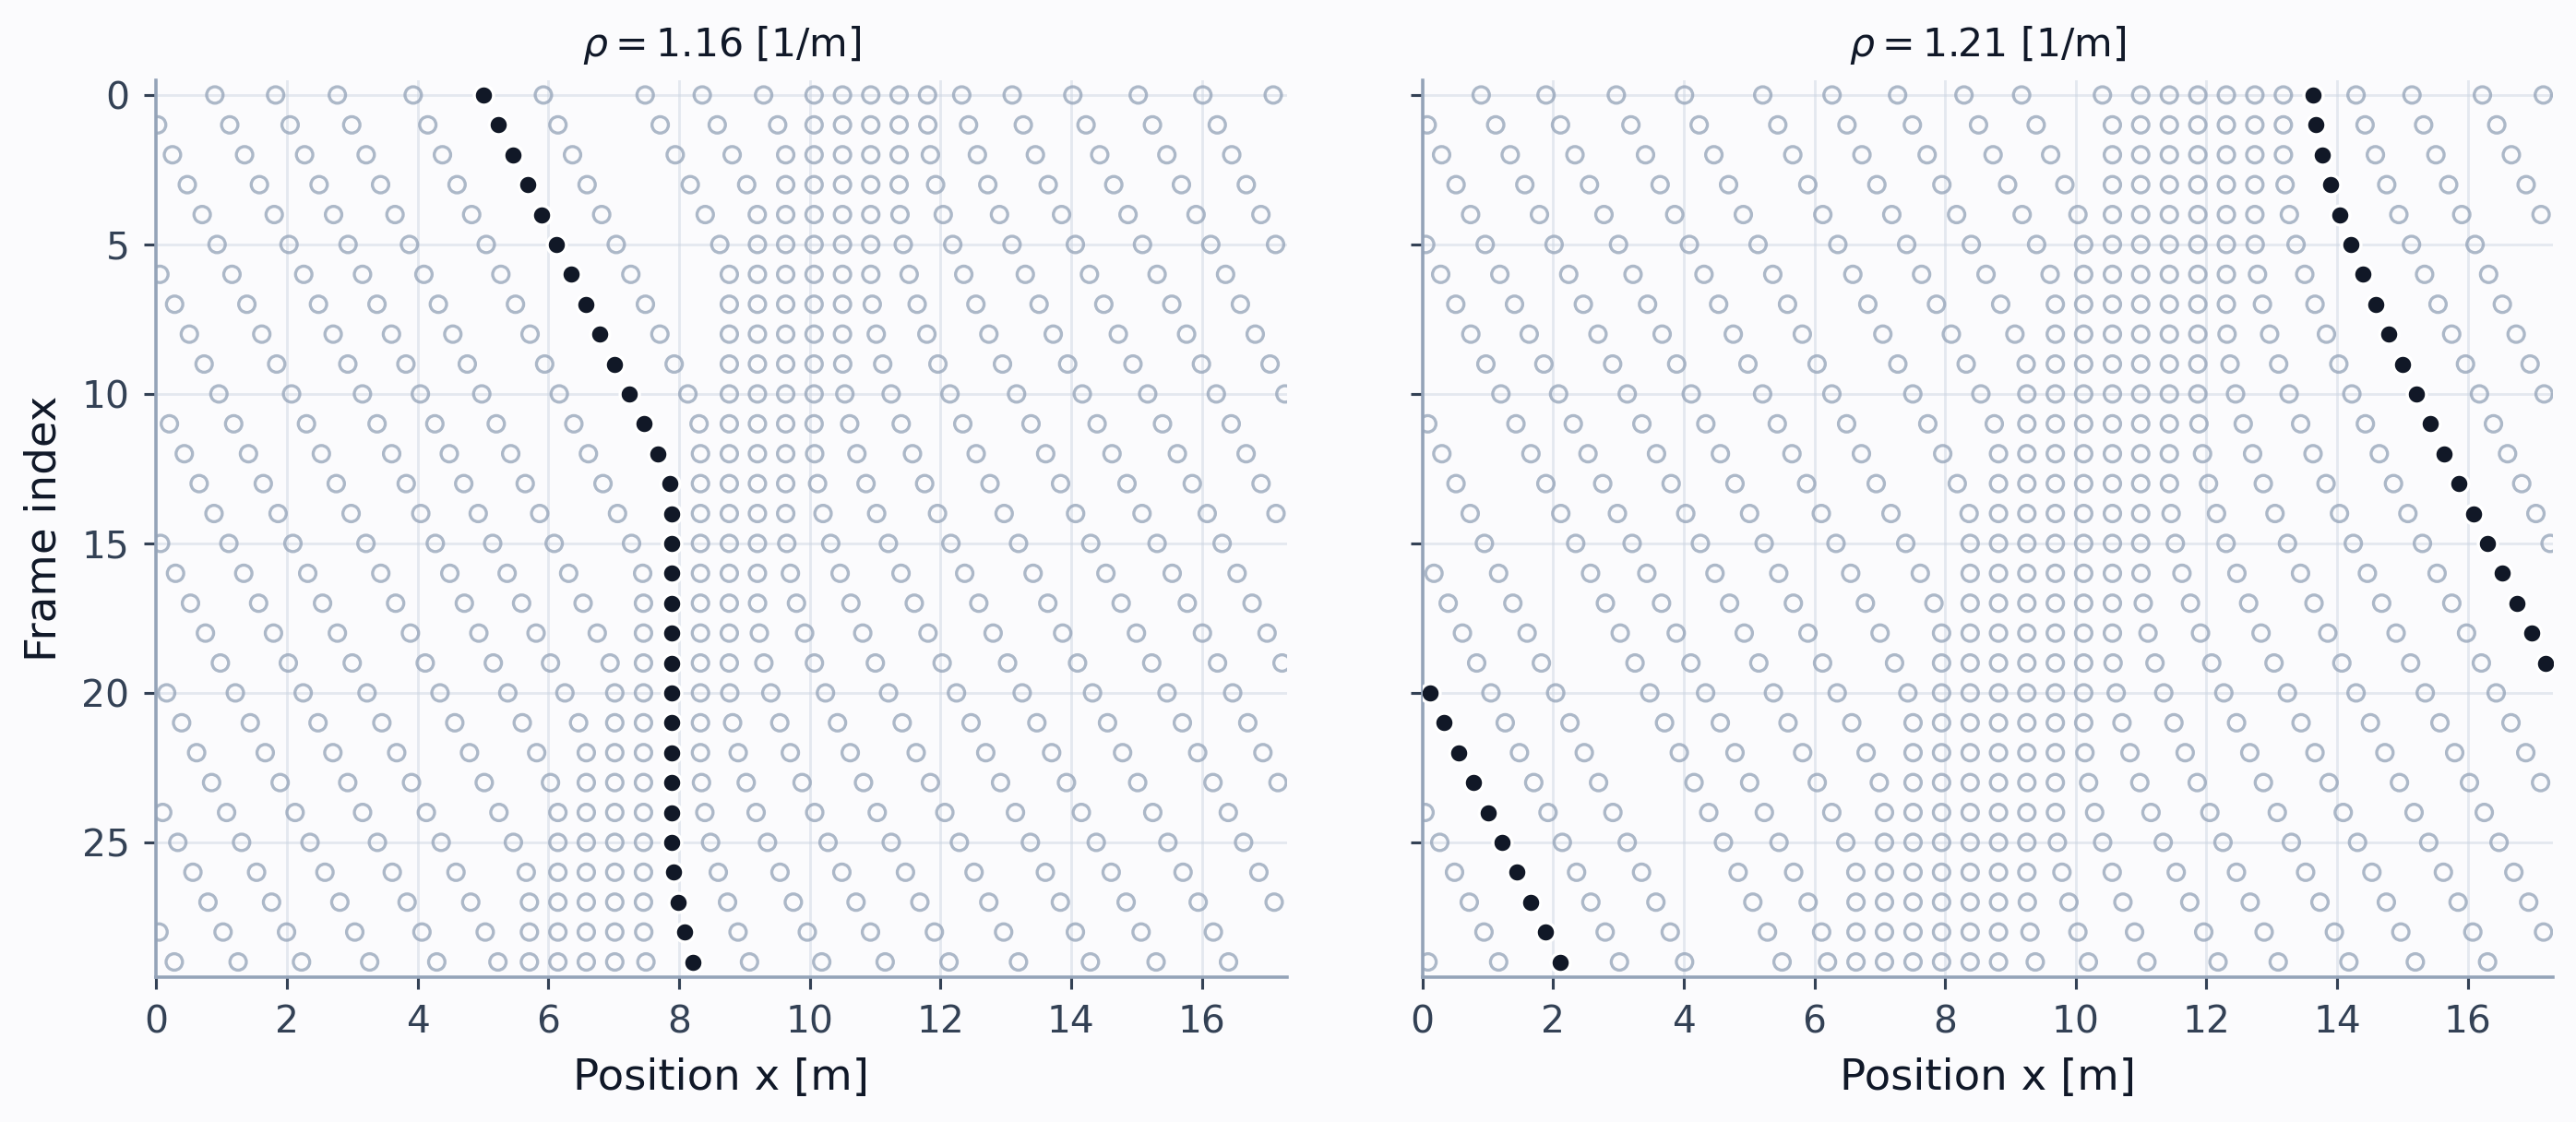
\includegraphics[width=0.96\linewidth, height=0.52\textheight, keepaspectratio]{stop_and_go.png}
\vspace{0.02cm}
{\scriptsize \par \emph{Fig 3: Same pedestrian tracked across $\rho=1.16$ and $\rho=1.21\,\mathrm{m}^{-1}$ ($b=0$).}}
\vspace{0.06cm}

\begin{columns}[T,onlytextwidth]
    \begin{column}{0.57\textwidth}
        \textbf{Instability \& Velocity Gap ($b=0$):}
        \begin{itemize}
            \item \textbf{Transition}: stable flow ($\rho=1.16$) $\rightarrow$ amplified perturbations ($\rho=1.21$).
            \item \textbf{Cascade}: leader slows $\rightarrow$ followers brake sharply $\rightarrow$ \textbf{backwards-propagating waves}.
        \end{itemize}
    \end{column}

    \begin{column}{0.40\textwidth}
        \begin{block}{Stabilization ($b > 0$)}
            Slower agents reduce required space $d(v)$, adding organic damping that suppresses artificial waves.
        \end{block}
    \end{column}
\end{columns}
\end{frame}

% : Section 6: Parameter Analysis :
\section{Parameter Analysis}
\begin{frame}{Parameter Analysis: New Sweep}
    \begin{itemize}
        \item \textbf{New varied parameter:} minimum required space $a$ in
        \[
            d_i(t)=a+bv_i(t).
        \]
        \begin{itemize}
            \item Keep $b=0.56\,\mathrm{s}$, $\tau=0.61\,\mathrm{s}$, and $L=17.3\,\mathrm{m}$ fixed.
            \item Sweep $a \in \{0.30, 0.36, 0.42\}\,\mathrm{m}$.
        \end{itemize}
        \item \textbf{Reason for this sweep:} $a$ changes the pedestrian's baseline footprint before any velocity-dependent spacing is added.
        \item \textbf{Question:} how much does this static footprint shift the onset of congestion?
    \end{itemize}
\end{frame}

\begin{frame}{Parameter Analysis: Minimum Required Space ($a$)}
\small
\begin{columns}[T,onlytextwidth]
    % Left Column: Diagram
    \begin{column}{0.5\textwidth}
        \centering
        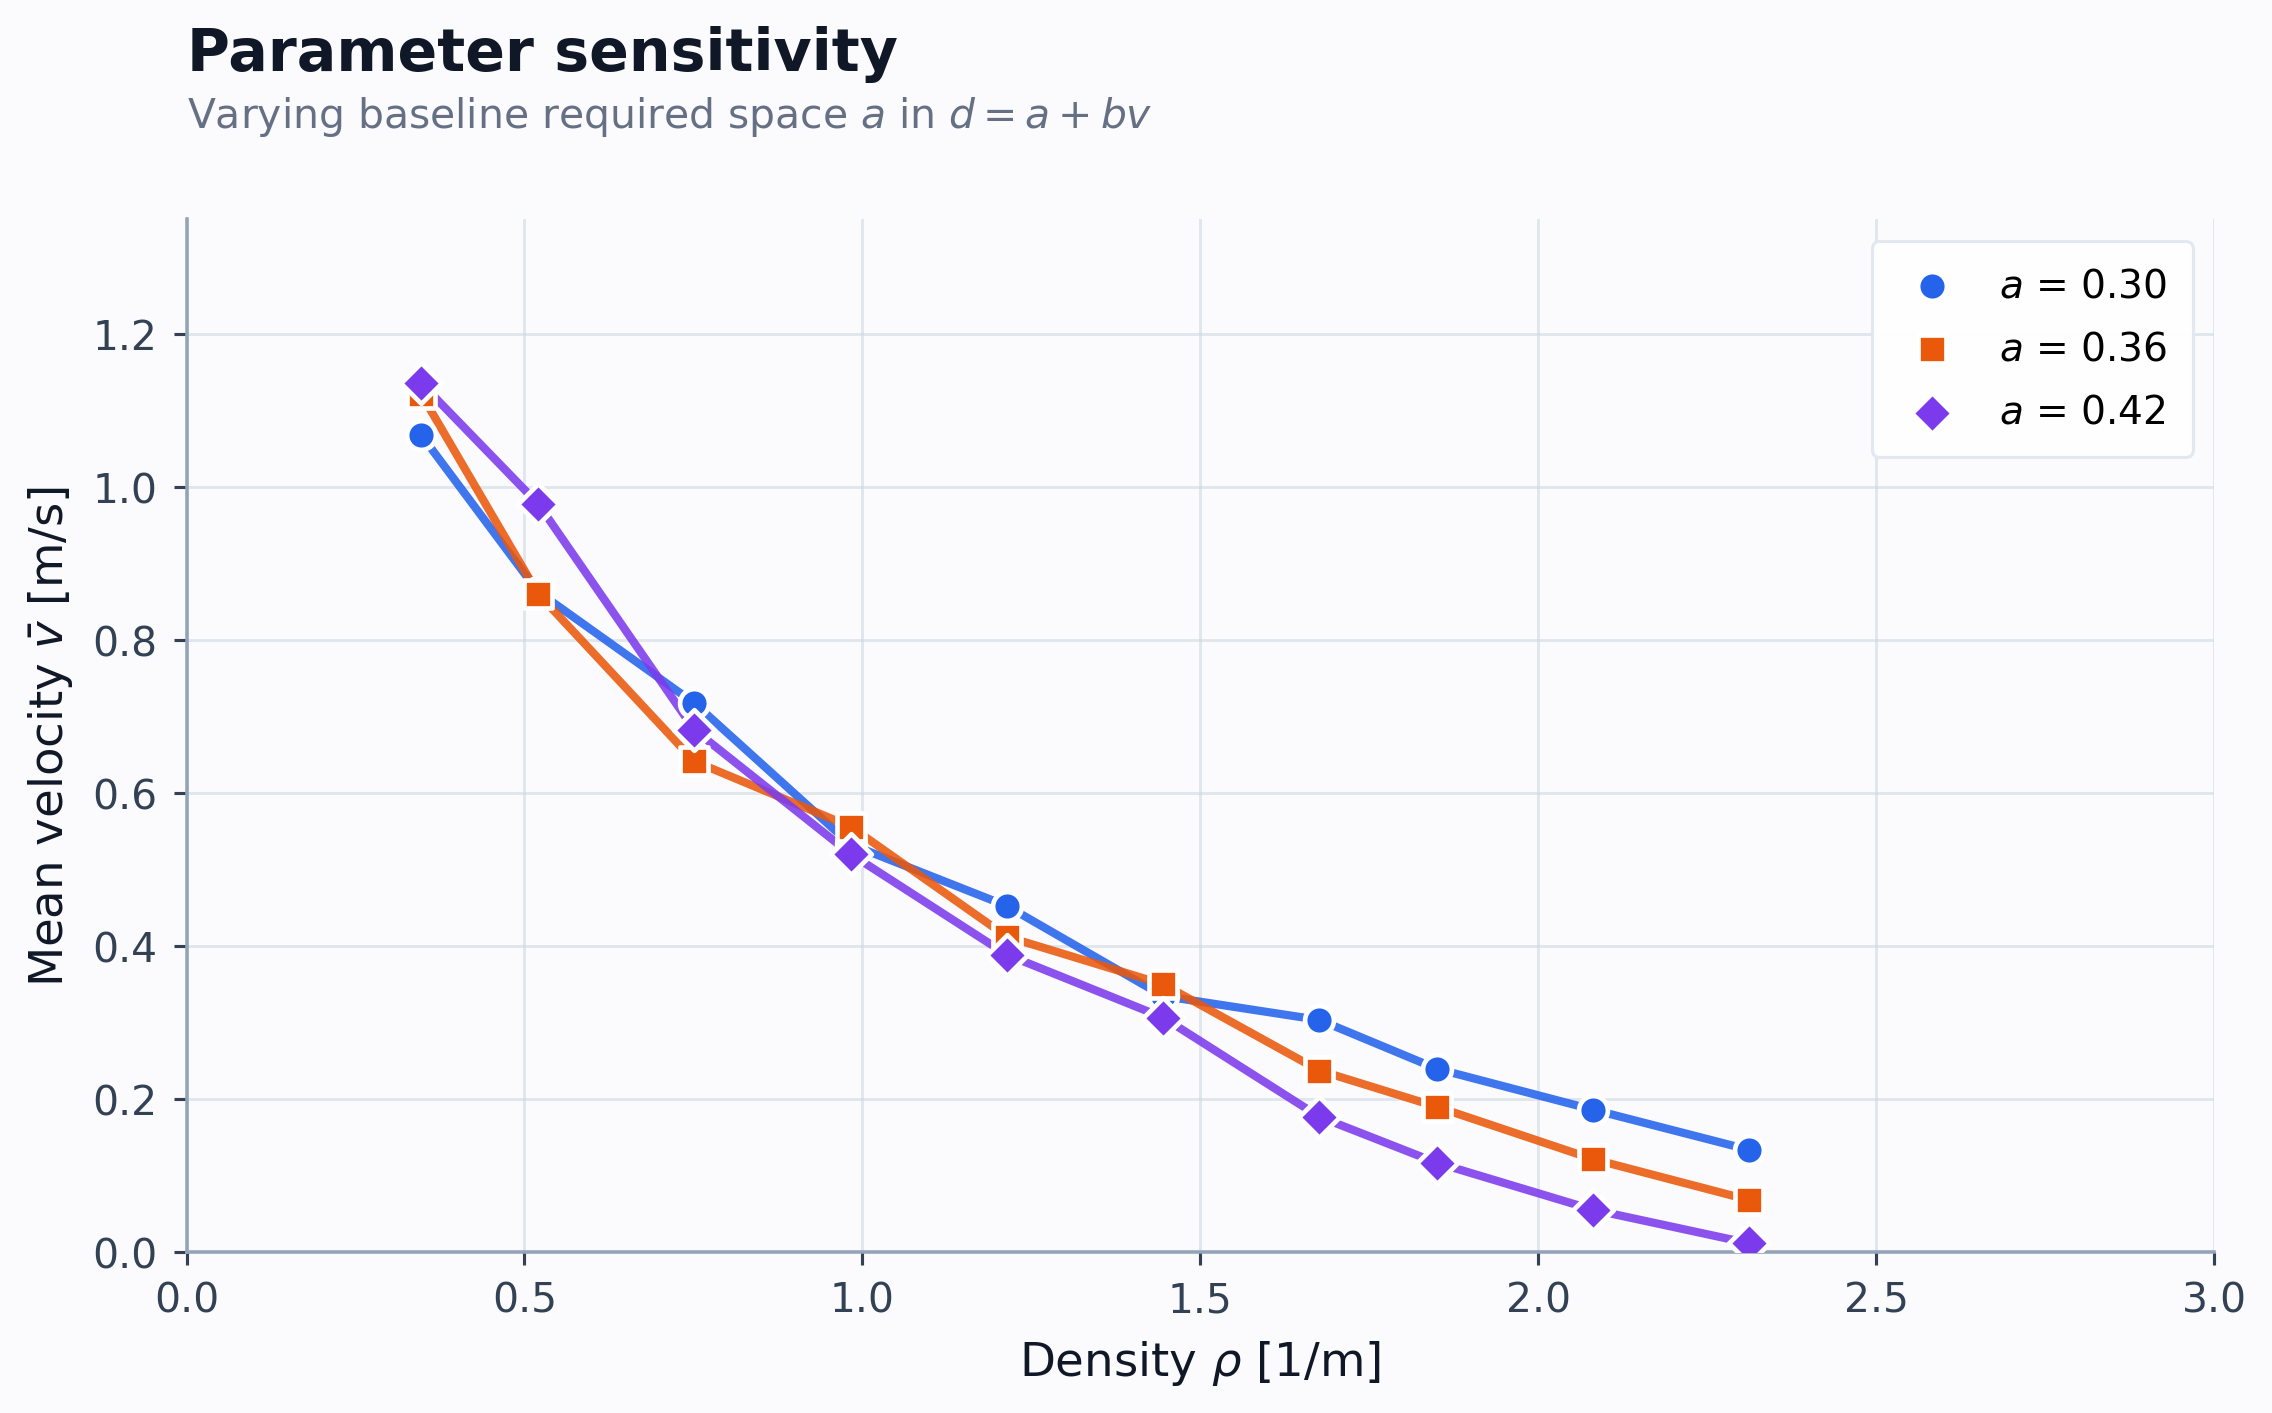
\includegraphics[width=\linewidth, height=0.65\textheight, keepaspectratio]{body_length.png}
        \vspace{0.1cm}
        {\scriptsize \par \emph{Fig 4: Fundamental diagram under different baseline spaces $a$.}}
    \end{column}

    % Right Column: Insights
    \begin{column}{0.48\textwidth}
        \textbf{Impact of Baseline Space:}
        \begin{itemize}
            \item \textbf{Low Density} ($\rho < 0.8\,\text{m}^{-1}$):
            \begin{itemize}
                \item Curves remain close.
                \item \textbf{Reason}: pedestrians rarely hit the hard-body constraint.
            \end{itemize}

            \vspace{0.3cm}

            \item \textbf{Medium--High Density}:
            \begin{itemize}
                \item Larger $a$ reduces free space earlier.
                \item The velocity drop shifts to lower densities.
            \end{itemize}
        \end{itemize}
    \end{column}
\end{columns}
\end{frame}

\begin{frame}{Parameter Analysis: Interpretation}
\small
\begin{columns}[T,onlytextwidth]
    \begin{column}{0.48\textwidth}
        \textbf{Physical Meaning of $a$:}
        \begin{itemize}
            \item $a$ is the non-negotiable body or personal-space baseline.
            \item It remains active even when pedestrians are almost stopped.
            \item Increasing $a$ lowers the effective packing capacity.
        \end{itemize}
    \end{column}

    \begin{column}{0.48\textwidth}
        \textbf{Model Consequence:}
        \begin{itemize}
            \item $b$ controls how spacing grows with speed.
            \item $a$ controls how early hard-body blocking starts.
            \item The fundamental diagram is therefore sensitive to both static and dynamic space terms.
        \end{itemize}

        \begin{block}{Key Finding}
            Calibrating $a$ changes congestion onset even when $b$ is fixed at the paper's best-fit value.
        \end{block}
    \end{column}
\end{columns}
\end{frame}

\section{Conclusion}

% --- Slide 6.1: Key Research Outcomes ---
\begin{frame}{Key Research Outcomes}
\footnotesize
\raggedright

\begin{columns}[T,onlytextwidth]
    % Left Column: Mathematical Enhancements
    \begin{column}{0.48\textwidth}
        \textbf{Model Reconstruction from Scratch:}
        \begin{itemize}
            \item \textbf{Directional constraints:} converted the 2D symmetric Social Force Model into a one-sided, forward-only 1D formulation.
            \item \textbf{Velocity bounds:} clamped velocities to $[0, v_i^0]$ to avoid backward motion and overshooting.
            \item \textbf{Dynamic required space:} Integrated speed-dependent required space $d_i(t) = a_i + b_i v_i(t)$.
        \end{itemize}
    \end{column}

    % Right Column: Macroscopic Verification
    \begin{column}{0.48\textwidth}
        \textbf{Macroscopic Verification:}
        \begin{itemize}
            \item \textbf{Convex curve recovery:} $b = 0.56\,\mathrm{s}$ restores the correct fundamental-diagram shape.
            \item \textbf{Wave damping:} $b > 0$ suppresses artificial stop-and-go waves under constant spacing.
            \item \textbf{Parameter sensitivity:} baseline space $a$ shifts congestion onset even with fixed $b$.
        \end{itemize}

        \begin{block}{Theoretical Validation}
            The model reproduces the macroscopic trend while exposing how required-space calibration changes the curve.
        \end{block}
    \end{column}
\end{columns}
\end{frame}


% --- Slide 6.2: Critical Insights & Future Work ---
\begin{frame}{Critical Insights \& Future Work}
\small
\raggedright

\begin{alertblock}{The $b$-Parameter Discrepancy}
    While empirical studies measure human safety headways at $b \approx 1.06\,\mathrm{s}$, the numerical calibration matches the macroscopic fundamental diagram at $b \approx 0.56\,\mathrm{s}$.
\end{alertblock}

\vspace{0.15cm}

\begin{columns}[T,onlytextwidth]
    % Left Column: Physical Cause (Why)
    \begin{column}{0.48\textwidth}
        \textbf{Identifying the Limitation:}
        \begin{itemize}
            \item \textbf{Model Short-Sightedness:} The 1D agents react \emph{exclusively} to their immediate predecessor.
            \item Lacking reaction delays or down-the-line anticipation, they can safely maintain tighter gaps ($b = 0.56\,\mathrm{s}$) without causing system collapse.
        \end{itemize}
    \end{column}

    % Right Column: Future Work (Where next)
    \begin{column}{0.48\textwidth}
        \textbf{Future Research Directions:}
        \begin{itemize}
            \item \textbf{Cognitive \& Behavioral Factors:} Incorporating human reaction delay times ($\Delta t_{\mathrm{reaction}} > 0$) and cognitive distraction parameters.
            \item \textbf{Multi-Anticipative Models:} Expanding the interaction scope to look several steps ahead ($i+2$, $i+3$), mimicking real human proactive gaze.
        \end{itemize}
    \end{column}
\end{columns}
\end{frame}

% Slide Final: Q&A
\begin{frame}
    \begin{center}
        \Huge THANK YOU!
        \vspace{0.5cm}
        \normalsize \\ Presented by Group 2
    \end{center}
\end{frame}

\end{document}
